\documentclass{report}
\usepackage{graphicx}
\usepackage{color}
\usepackage[colorlinks,urlcolor=blue,linkcolor=black,citecolor=blue]{hyperref}

\begin{document}

\title{Metasploit 3.0 Developer's Guide}
\author{skape}

\begin{titlepage}
    \begin{center}
        \huge{{Metasploit 3.0 Developer's Guide}} \\[150mm]
        \rule{10cm}{1pt} \\[8mm]
        \small\bf{skape} \\
        \small\bf{mmiller@hick.org} \\[4mm]
        \textit{Last modified: \small{11/24/2003}}
    \end{center}
\end{titlepage}

\tableofcontents

\setlength{\parindent}{0pt} \setlength{\parskip}{8pt}

\chapter{Introduction}

\par
The Metasploit framework is an open-source exploitation framework
that is designed to provide security researches and pen-testers with
a uniform model that allows for the rapid development of exploits,
payloads, encoders, NOP generators, and reconnaissance tools.  The
framework provides exploit writers with the ability to re-use large
chunks of code that would otherwise have to be copied or
re-implemented on a per-exploit basis.  To help further this cause,
the Metasploit staff is proud to present the next major evolution of
the exploitation framework: version 3.0.

\par
The 3.0 version of the framework is a re-factoring of the 2.x branch
which has been written entirely in Ruby.  The primary goal of the
3.0 branch is to make the framework easy to use and extend from a
programmatic aspect.  This goal encompasses not only the development
of framework modules, such as exploits, but also to the development
of third party tools and plugins that can be used to increase the
functionality of the entire suite.  By developing an easy to use
framework at a programmatic level, it follows that exploits and
other extensions should be easier to understand and implement than
those provided in earlier versions of the framework.

\par
This document will provide the reader with an explanation of the
design goals, methodologies, and implementation details of the 3.0
version of the framework.  Henceforth, the 3.0 version of the
framework will simply be referred to as \textit{the framework}.

    \section{Why Ruby?}

\par
During the development of the framework, the one recurring question
that the Metasploit staff was continually asked was why Ruby was
selected as the programming language.  To avoid having to answer
this question on an individual basis, the authors have opted for
explaining their reasons in this document.

\par
The Ruby programming language was selected over other choices, such
as python, perl, and C++ for quite a few reasons.  The first, and
primary, reason that Ruby was selected was because it's a language
that the Metasploit staff enjoyed writing in.  After spending time
analyzing other languages and factoring in past experiences, the
Ruby programming language was found to offer both a simple and
powerful approach to an interpreted language.  The degree of
introspection and the object-oriented aspects provided by Ruby was
something that fit very nicely with some of the requirements of the
framework, where automated class construction and for the purpose of
code re-use was a very key concern, and it was one that perl was not
very well suited to offer. On top of this, the syntax is incredibly
simplistic and provides the same level of language features that
other more accepted languages have, like perl.

\par
The second reason Ruby was selected was because of its platform
independent support for threading.  While a number of limitations
have been encountered during the development of the framework under
this model, the Metasploit staff has observed a marked performance
and usability improvement over the 2.x branch.  Future versions of
Ruby (the 1.9 series) will back the existing threading API with
native threads for the operating system the interpreter is compiled
against which will solve a number of existing issues with the
current implementation, such as permitting the use of blocking
operations.  In the meantime, the existing threading model has been
found to be far superior to a forking model, especially on platforms
that lack a native fork implementation like Windows.

\par
Another reason that Ruby was selected was because of the supported
existence of a native interpreter for the Windows platform.  While
perl has a cygwin version and an ActiveState version, both are
plagued by usability problems.  The fact that the Ruby interpreter
can be compiled and executed natively on Windows drastically
improves performance.  Furthermore, the interpreter is also very
small and can be easily modified in the event that there is a bug.

\par
The Python programming language was also a language candidate. The
reason the Metasploit staff opted for Ruby instead of Python was for
a few different reasons.  The primary reason is a general distaste
for some of the syntactical annoyances forced by Python, such as
block-indention.  While many would argue the benefits of such an
approach, some members of the Metasploit staff find it to be an
unnecessary restriction.  Other issues with Python center around
limitations in parent class method calling and backward
compatibility of interpreters.

\par
The C/C++ programming languages were also very seriously considered,
but in the end it was obvious that attempting to deploy a portable
and usable framework in a non-interpreted language was something
that would not be feasible.  Furthermore, the development time-line
for this language selection would most likely be much longer.

\par
Even though the 2.x branch of the framework has been quite
successful, the Metasploit staff encountered a number of limitations
and annoyances with perl's object-oriented programming model, or
lack thereof.  The fact that the perl interpreter is part of the
default install on many distributions is not something that the
Metasploit staff felt was worth detouring the language selection.

\chapter{Architecture and Design}

\par
The framework was designed to be as modular as possible as to
encourage the re-use of code across various projects.  The most
fundamental piece of the architecture is the \textit{Rex} library
which is short for the \texttt{Ruby Extension Library}\footnote{This
library has many similarities to the 2.x Pex library}. Some of the
components provided by Rex are a wrapper socket subsystem,
implementations of protocol clients and servers, a logging
subsystem, exploitation utility classes, and a number of other
useful classes.  Rex itself is designed to have no dependencies
other than what comes with the default Ruby install. In the event
that a Rex class depends on something that is not included in the
default install, the failure to find such a dependency should not
lead to the inability to use Rex.

\par
The framework itself is broken down into a few different pieces, the
most low-level being the \textit{framework core}.  The framework
core is responsible for implementing all of the required interfaces
that allow for interacting with exploit modules, sessions, and
plugins. This core library is extended by the \textit{framework
base} which is designed to provide simpler wrapper routines for
dealing with the framework core as well as providing utility classes
for dealing with different aspects of the framework, such as
serializing module state to different output formats.  Finally, the
base library is extended by the \textit{framework ui} which
implements support for the different types of user interfaces to the
framework itself, such as the command console and the web interface.

\par
Separate from the framework are the modules and plugins that it's
designed to support.  A framework module is defined as being one of
an exploit, payload, encoder, NOP generator, or recon tool. These
modules have a well-defined structure and interface for being loaded
into the framework.  A framework plugin is very loosely defined as
something that extends the functionality of the framework or
augments an existing feature to make it act in a different manner.
Plugins can add new commands to user interfaces, log all network
traffic, or perform whatever other action might be useful.

\par
Figure \ref{fig-arch-pkg} illustrates the framework's inter-package
dependencies.  The following sections will elaborate on each of the
packages described above and the various important subsystems found
within each package.

\begin{figure}[h]
\begin{center}
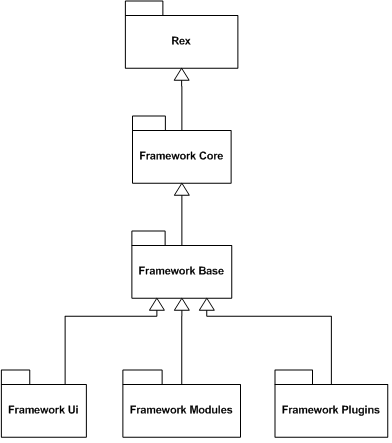
\includegraphics[height=4in,width=4in]{dev_guide_arch_packages}
\caption{Framework 3.0 package dependencies} \label{fig-arch-pkg}
\end{center}
\end{figure}

    \section{Rex}
        \subsection{Logging}
        \subsection{Protocols}
        \subsection{Services}
        \subsection{Socket}
        \subsection{Synchronization}
        \subsection{Exploitation}
    \section{Framework Core}
        \subsection{Framework Managers}
        \subsection{Event Notifications}
    \section{Framework Base}
        \subsection{Simplified Framework}
        \subsection{Configuration}
        \subsection{Logging}
        \subsection{Serialization}
    \section{Framework Ui}
        \subsection{Console}
        \subsection{Web}
\chapter{Framework Modules}
    \section{Encoder}
    \section{Exploit}
        \subsection{Types}
        \subsection{Stances}
        \subsection{Mixins}
    \section{Nop}
    \section{Payload}
        \subsection{Single}
        \subsection{Stager}
        \subsection{Stage}
    \section{Recon}
        \subsection{Discoverer}
        \subsection{Analyzer}
\chapter{Framework Plugins}
    \section{User-interface Plugins}
\chapter{Methodologies}
    \section{Writing an Exploit}
\chapter{Conclusion}

\end{document}
